\subsubsection{Mediciones con códigos QR}

Dentro de una imagen podemos tener miles de referencias por las cual guiarnos o tomar como objetivo para establecer una referencia de la ubicación de la cámara, una buena alternativa nos pareció el uso de códigos QR que en su payload contengan información relevante sobre la ubicación del objeto, entonces, si dentro de las varias fotos que capturamos realizando una trayectoria podemos identificar códigos QR en ellas, el procesamiento de imágenes se centra en la tarea puntual de identificar los códigos, y por lo tanto es más rápida y menos pesada computacionalmente.

Ya especificamos en secciones anteriores que al mapa del robot lo proyectamos sobre una superficie en dos dimensiones con distintas celdas que podemos identificar mediante un sistema de ejes cartesianos. Teniendo una referencia a gran escala de su ubicación podemos determinar fácilmente en qué parte del mapa se encuentra ya que van a ser un par coordenadas en el eje $X$ y el eje $Y$. Si a este par de coordenadas lo colocamos como payload dentro del código QR, vamos a poder identificar donde se encuentra el robot o al menos tener una referencia real de donde puede llegar a encontrarse.

Esto por supuesto no es suficiente ya que al ser una referencia generalizada, no obtenemos una precisión de la cual confiarnos. Es por ello que decidimos medir la distancia hacia el código QR, tanto en el eje $X$ como en el eje $Y$, sabiendo que si el robot se encuentra posicionado de forma central con el código QR, se encuentra exactamente ubicado donde marca el par de ejes cartesianos.

Para las pruebas y la determinación de los parámetros al calcular una distancia efectiva a las cuales se pueden detectar los códigos QR se tomó un objetivo fijo con distintas ya definidas y a partir de ahí poder determinar cual es la distancia mínima de reconocimiento. Se implemento la siguiente experiencia para determinar los parámetros de la cámara.

\begin{figure}[H]
   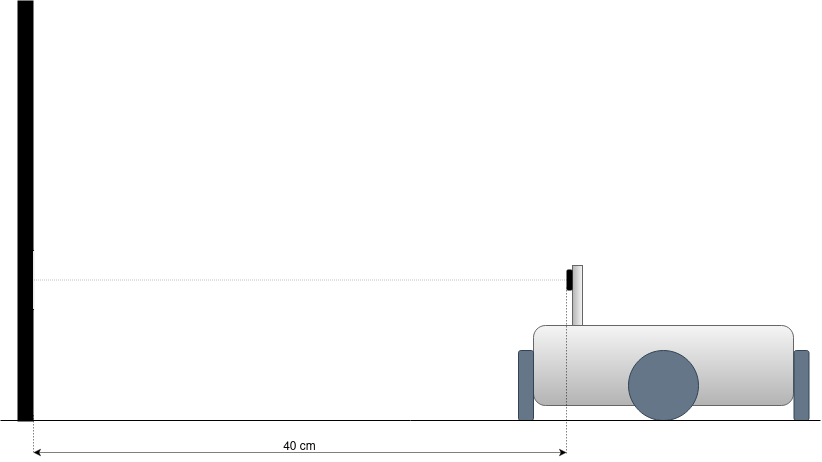
\includegraphics[trim={0 0 0 6cm}, clip, width=1.0\linewidth]{images/robot_medicion_qr.png}
   \caption{Experiencia para la obtención de parámetros de calibración de la cámara}
   \label{fig:robot_medicion_qr}
\end{figure}

El objetivo de esta calibración es encontrar la longitud focal, la cual es una constante que representa la distancia desde el centro del lente objetivo hasta el sensor de imagen. Siempre tomando como el ejemplo dimensiones de las fotografías obtenidas por la ESP32 las cuales se detallan en la siguiente imagen y donde el ancho es de $1280px$ mientras tanto que el alto es de $720px$.

\begin{figure}[H]
   \centering
   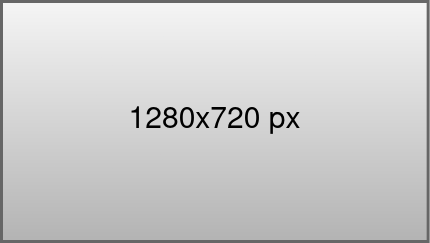
\includegraphics[width=0.5\linewidth]{images/ejemplo_foto.drawio.png}
   \caption{Ejemplo de las dimensiones tomadas por la cámara}
   \label{fig:qr}
\end{figure}

Por lo tanto se calcula de la siguiente manera \cite{wu2018size}:

\begin{equation}
   Longitud\ focal [px] = \frac{Ancho\ del\ QR\ en\ la\ imagen\ [px] \times Distancia\ real\ [mm]}{Dimensi\acute{o}n\ real\ del\ c\acute{o}digo\ QR\ [mm]}
   \label{ec:logitud_focal}
\end{equation}

Donde:
\begin{itemize}
   \item El ancho del QR en la imagen se representa en cantidad de pixeles.
   \item La distancia real es entre el código QR y la cámara medida en milímetros, en este caso 400$[mm]$.
   \item La dimensión real del código QR es el ancho del código QR, en este caso es de 50$[mm]$.
\end{itemize}

Al consultar el tamaño de pixel dado por la hoja de datos de la cámara OV2640, obtenemos que es de $2.2\mu m$. Por lo que podemos convertir la longitud focal de $[px]$ a $[mm]$ mediante la siguiente expresión:

\begin{equation}
 Longitud\ focal [mm] = Longitud\ focal [px] \times Dimensi\acute{o}n\ del\ pixel [mm/px]
\end{equation}

Una vez obtenido este parámetro lo vamos a utilizar para comparar la dimensión en píxeles del código QR en la imagen con el código QR en sí, y de esa manera obtener la distancia que existe hacia el objeto con la fórmula:

\begin{equation}
   Distancia[mm] = \frac{Dimensi\acute{o}n\ real\ del\ c\acute{o}digo\ QR\ [mm] \times Longitud\ focal\ [px]}{Ancho\ del\ QR\ en\ la\ imagen\ [px]}
   \label{ec:distancia_qr}
\end{equation}

Por supuesto que esto se aplica únicamente cuando en la fotografía se logra identificar un código QR, si durante el procesamiento de la imagen esto no sucede, no se va a poder determinar la distancia. Realizando varias pruebas se logró determinar que si la cámara se encuentra entre los $500mm$ y $600mm$ del objetivo, el código QR es identificable en la imagen. Una distancia mayor al rango descrito ya se considera fuera del rango.

A partir del posicionamiento del robot se obtuvo la siguiente imagen, la cual se usó de referencia para medir la distancia en todas las demás fotografías utilizando las expresiones desarrolladas anteriormente.

\begin{figure}[H]
   \centering
   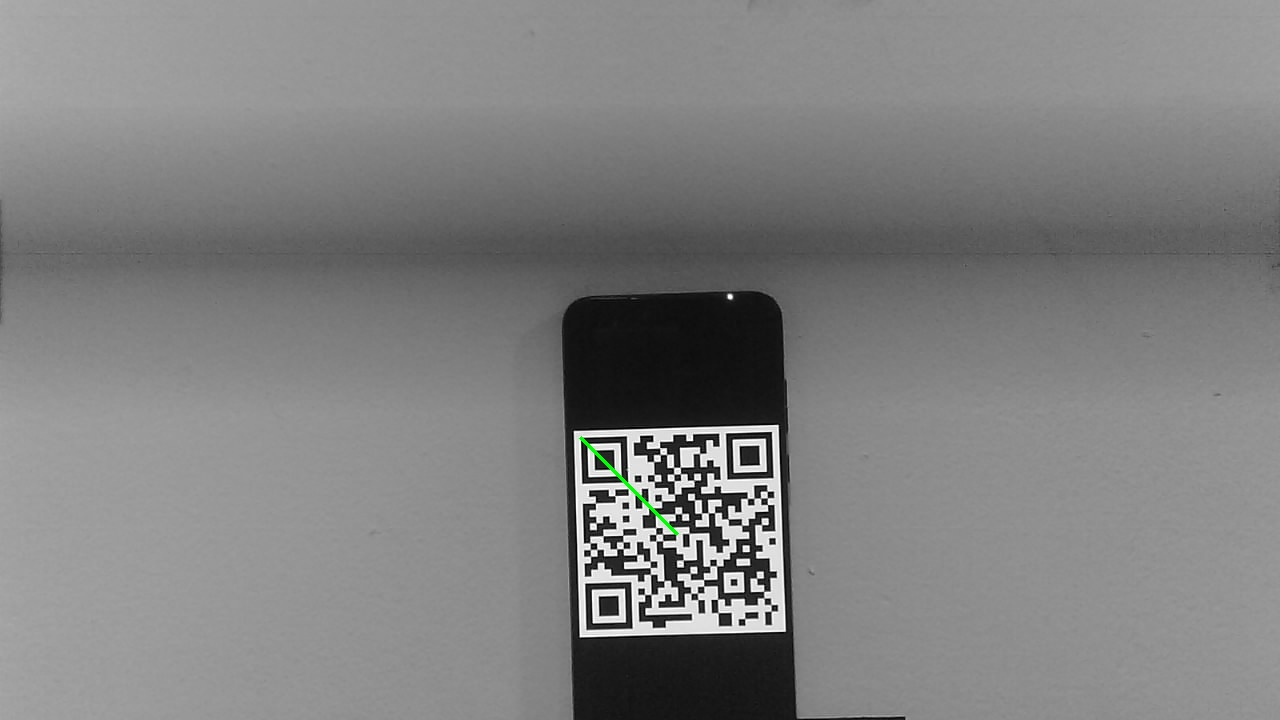
\includegraphics[width=0.8\linewidth]{images/img_centro.jpg}
   \caption{Imagen de referencia obtenida por el robot}
   \label{fig:img_centro}
\end{figure}